\part{Spécification}

\section{Caractéristiques}
\subsection{Périphériques requis}
Périphériques :
\begin{itemize}
	\item Un souris deux bouton.
	\item Un clavier standart.
	\item Un terminal pouvant afficher au moins 80 car/ligne, 50 lignes/page + les quatres lignes appartenant à l'interface de l'éditeur.\\
\end{itemize}

L'éditeur de texte ne gère qu'un seul encodage : l'\textbf{ASCII étendu}.

\subsection{Zone tampon}
Cette zone mémoire contient la dernière sélection effectuée.

\section{Comportement de l'interface}

\paragraph{Curseur :} Le curseur est un rectangle semi-transparent,de la hauteur d'une ligne, de la largeur d'un caractère, et pouvant être déplacé via un clic de la souris. Il ne peut être placé que sur un caractère existant ou en début de ligne.

\paragraph{Ligne d'entête :} Elle affiche le nom du fichier, son état, le numéro de la page en édition, le numéro de la ligne et de la colonne où se trouve le curseur, et eventuellement le mode de lecture (lecture seule ou lecture/écriture).

Un fichier ne peut être que dans 2 états :
\begin{itemize}
	\item Enregistré : La version affichée à l'écran et la version sur le disque sont les même.
	\item Modifié :	La version affichée à l'écran et la version sur le disque sont différentes.
\end{itemize}

\paragraph{Zone de saisie :} Cette zone, reservée à la saisie du texte, fait :
\begin{itemize}
	\item 80 caractères de large
	\item 50 lignes de haut
\end{itemize}
C'est la dimension d'une page \emph{affichée}.\\

Si l'utilisateur dépasse :
\begin{itemize}
	\item 80 caractères : Le nouveau caractère est transféré sur la ligne suivante. Aucun saut de ligne n'est cependant ajouté, seul l'affichage est modifié.
	\item 50 lignes : L'éditeur insère un caractère de fin de page et place le curseur au début de la page suivante.\\
\end{itemize}

Dans cette zone, l'utilisateur peut insérer du texte en tapant les caractères qu'il veut insérer au clavier. Les caractères saisis seront placés avant le curseur. Le caractère de fin de ligne est inséré par la touche \og Entrée\fg.

L'utilisateur peut sélectionner du texte en appuyant sur le bouton de la souris, en déplacant le curseur jusqu'au dernier caractère de la sélection, puis en relachant le bouton. Le texte sélectionné est automatiquement mis en zone tampon.

L'utilisateur peut aussi coller au niveau du curseur le texte présent dans la zone tampon (\textsl{i.e} le dernier texte sélectionné ) en appuyant sur le second bouton de sa souris.

L'utilisateur peut supprimer le caractère courant en appuyant sur la touche standart \og Suppr\fg. Il peut aussi supprimer le texte sélectionné au curseur en sélectionnant le texte, puis en appuyant sur la touche standart \og Suppr\fg.

\paragraph{Page glissante :}
L'utilisateur a aussi la possibilité de naviguer entre les pages en appuyant sur les flèches directionnelles du clavier :
\begin{itemize}
	\item \og Flêche haut\fg : Change la page courante avec la page précédente si elle existe.
	\item \og Flêche bas\fg : Change la page courante avec la page suivante si elle existe.
\end{itemize}
Dans les deux cas, le curseur est placé en première ligne.

\paragraph{Menu contextuel}
Constitué de 3 lignes, une \textsl{ligne de saisie} et deux lignes d'aide contextuel, il repertorie toutes les commandes accessibles dans le contexte courant sous la forme :
TODO INSËRER SNITPPET

Les différents éléments de l'aide :
\begin{itemize}
	\item \textbf{Charger} : \og CTRL + o\fg
	\item \textbf{Enregistrer} : \og CTRL + s\fg
	\item \textbf{Fin de page} : \og CTRL + p\fg
	\item \textbf{Quitterr} : \og CTRL + q\fg
\end{itemize}

Dans le cas où les commandes de gestion de fichiers sont appelée, l'aide contextuelle affiche (dans le cas d'un système en Français) :\\
\begin{center}
\fbox{
\begin{tabular}{ll}
	Veuillez saisir le chemin absolu du fichier &~\\
	Enter: Valider & ESC : Annuler\\
\end{tabular}
}
\end{center}
~\\
Toutes les saisies relatives aux noms de fichiers seront effectuée dans la \textsl{ligne de saisie}.

\paragraph{Gestion des fichiers :}
L'utilisateur peut charger un fichier existant en appuyant simultanément sur les touches \og CTRL + O\fg. Dans ce cas, le programme demande à l'utilisateur de saisir le chemin absolu du fichier à ouvrir dans la ligne de saisie.

Il peut aussi sauvegarder le texte en cours d'édition. Il est demandé à l'utilisateur de saisir le chemin absolu du nouveau fichier. Si le nom de fichier est le même que celui qui est en cours d'édition, les modifications sont apporées sur le fichier déjà sauvegardé.

\paragraph{Gestion des langues :}
La langue de l'éditeur, \textsl{i.e.} les message d'erreur et les messages du menu contextuel, prend automatiquement celle du système.

\subsection{Lancement}
Deux modes de lancement sont disponibles :
\begin{enumerate}
	\item Sans paramètre : Un fichier vide appelé \og Untitled\fg est ouvert, mais pas enregistré.
	\item Avec un paramètre : Le fichier passé en paramètre est chargé et affiché s'il existe.
\end{enumerate}

\section{Diagramme comportemental}
\begin{figure}[H]
\begin{center}
    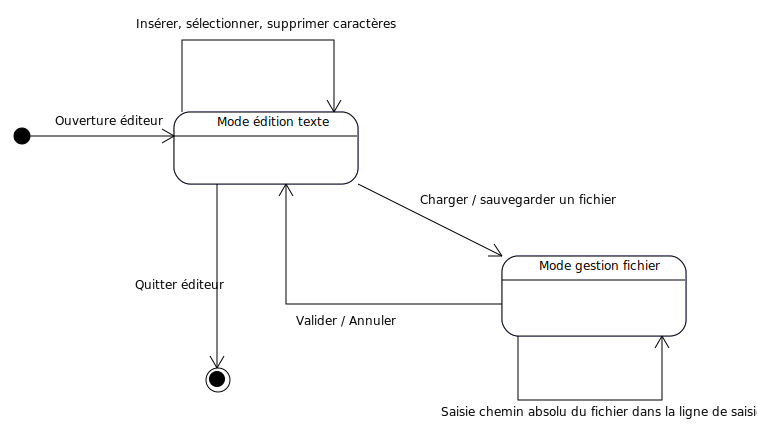
\includegraphics[width=13cm]{img/EtatsEditeur}
	\vspace{-1cm}
\end{center}
\end{figure}

\section{Interface utilisateur}
\begin{figure}[H]
\begin{center}
    \includegraphics[width=15cm]{img/MOD-Edit}
	\vspace{-1cm}
\end{center}
\end{figure}

\section{Liste des erreurs}
Seules les opérations sur les fichiers peuvent générer des erreurs. Les messages dépendent de la langue du système. Ici pour un système un Français :

\paragraph{Le nom de fichier à charger n'existe pas :} Le menu contextuel affiche \og Fichier inexistant\fg
\paragraph{Le fichier où aura lieux la sauvegarde est protégé en écriture :} Le menu contextuel affiche \og Fichier protégé\fg

\section{Bilan}
Tout en respectant un cahier des charges réaliste, notre application a le mérite de proposer toutes les fonctions de bases pour manipuler un document source. Il permet, dans un contexte \emph{multilangue}, avec des \emph{requis matériels minimalistes}, quelque soit le \emph{système d'exploitation}, ou la \emph{machine cible} :
\begin{itemize}
	\item D'effectuer toutes les opérations de fichiers du type : Ouvrir, charger, sauvegarder
	\item D'insérer, modifier, supprimer du texte
	\item De naviguer dans un fichier texte, au travers de ses différentes pages
\end{itemize}
